\documentclass[11pt,fleqn,a4paper]{article}
\usepackage[ngerman]{babel}
\usepackage[utf8]{inputenc}
\usepackage{textcomp}
\usepackage{graphicx}
\usepackage{upgreek}
\usepackage{floatflt}
\usepackage{amsmath}
\usepackage{amssymb}
\usepackage[final]{pdfpages}
\usepackage[a4paper, left=2cm, right=2cm, top=2cm]{geometry}
\usepackage[T1]{fontenc}
\usepackage{lmodern}
\renewcommand*\familydefault{\sfdefault}


\title{Grundbau Beleg}
\author{Paul Debus \and Matrikelnummer: 110113}

\begin{document}
\pagenumbering{roman}
\maketitle
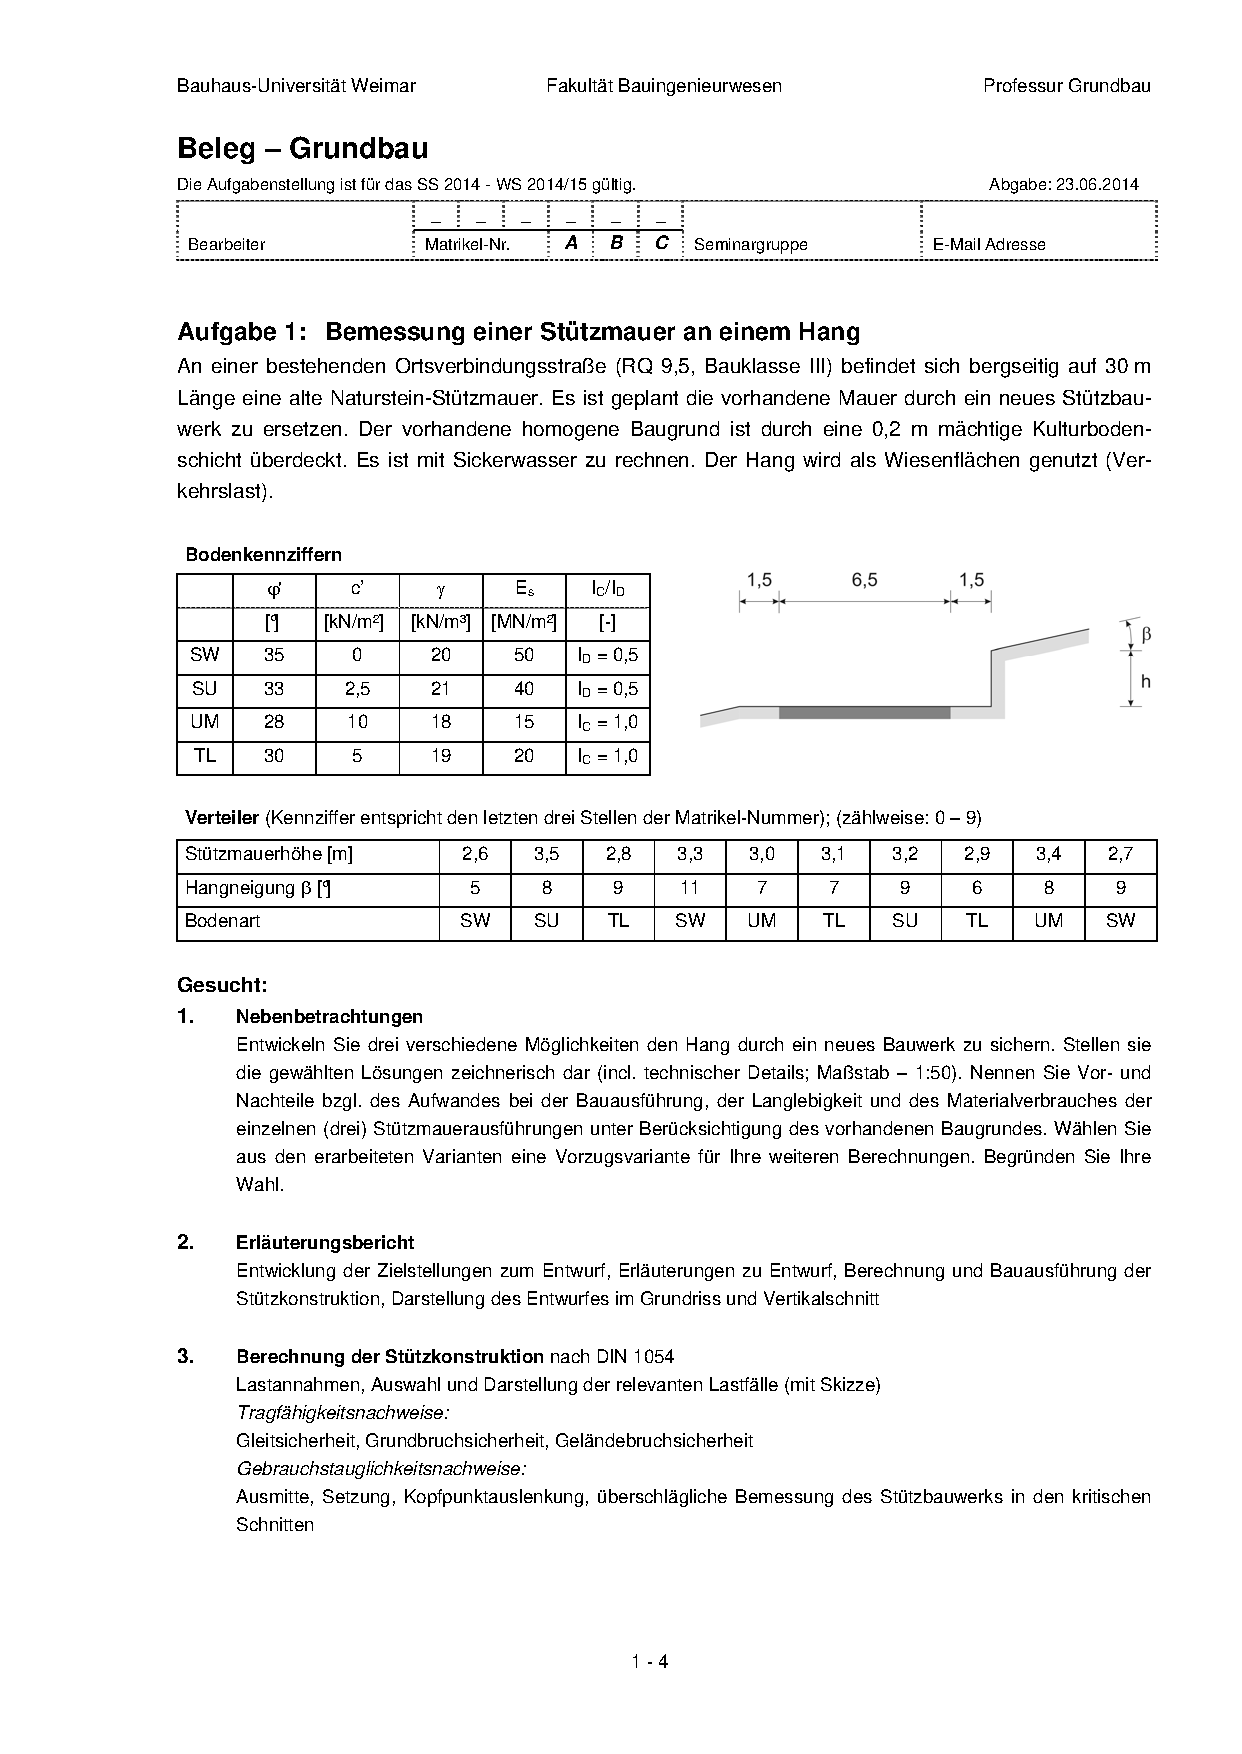
\includepdf[pages=1,pagecommand=\section{Aufgabenstellung}, scale=0.9]{aufgabe.pdf}
\includepdf[pages=2-,pagecommand={},scale=0.9]{aufgabe.pdf}
\tableofcontents
\newpage
\pagenumbering{arabic}
\section{Aufgabe 1}
\subsubsection*{Festlegung der eigenen Parameter aus Verteiler}
Matrikelnummer 110113
\begin{itemize}
\item Stützmauerhöhe 3,3m
\item Hangneigung $11^\circ$
\item Bodenart SW
\item $\varphi $' = $35^\circ$
\item c' = 0 [kN/m²]
\item $\gamma$ = 20 [kN/m³]
\item $E_s$ = 50 [MN/m²]
\item $l_c/l_o$ = 0.5
\end{itemize}
\subsection{Erläuterungsbericht}
\subsubsection*{Charakteristik der Aufgabe und des Standortes}
Es soll eine 30m lange Stützmauer entlang einer Straße erneuert werden. Dazu soll die vorhandene Natursteinmauer durch ein neues Bauwerk ersetzt werden. Der anstehende Boden ist ein abgestufter Kies, der von 0.2m Mutterboden bedeckt wird. Der Hang wird als Wiese genutzt und es mit Sickerwasser zu rechnen. \\
Im folgenden werden drei Varianten für das neue Bauwerkt beschrieben, von denen dann eine ausgewählt und bemessen wird.
\subsubsection*{Variante 1: Spundwand} 
Eine Spundwand ist ein in den Boden gerammtes Stahlprofil, welches als wie ein Kragträger wirkt. Durch den guten Verbund der einzelnen Elemente, sind Spundwände praktisch wasserdicht. Ab einer gewissen Höhe verankert man Spundwände horizontal in den Boden um Verformungen und Momente in der Baugrubensohle zu reduzieren und damit die Einbindelänge. Spundwände werden vor allem für den Baugrubenverbau eingesetzt, da sie sehr schnell zu montieren sind und nach dem Abbau wieder verwendet werden können. Für dauerhafte Bauten werden Spundwände besonders im Hafenbau eingesetzt, aber auch im Straßenbau zur Hangsicherung. \\
Der Aufwand bei der Bauausführung ist sehr gering, da die Spundwand einfach hinter der schon bestehenden Wand eingerammt werden kann und man diese danach abtragen kann. Bei anderen Befestigungen wie z.B. einer Winkelmauer ist eine Baugrube erforderlich, die allein schon eine Spundwand zur Absicherung braucht. Der Montageaufwand ist daher im Vergleich zu anderen Verfahren sehr gering. \\
Da Spundwände aus Stahl hergestellt werden, muss sich auch um Korrosionsschutz Gedanken gemacht werden. Gerade auf der Seite des anstehenden Bodens ist dieser nur sehr schwer zu leisten, sodass eine Spundwand nicht verlässlich vor Korrosion geschützt werden kann. Da ein Dauerbauwerk auf mehrere Jahrzehnte ausgelegt wird (wenn nicht sogar noch länger), wird es irgendwann zu Einschränkungen der Tragfähigkeit einer Spundwand kommen. \\
Für kurzzeitige Verbaue sind Spundwände sehr gut geeignet, bei Dauerbauwerken kann man Probleme mit der Haltbarkeit bekommen.
\newpage
\begin{figure}[h]
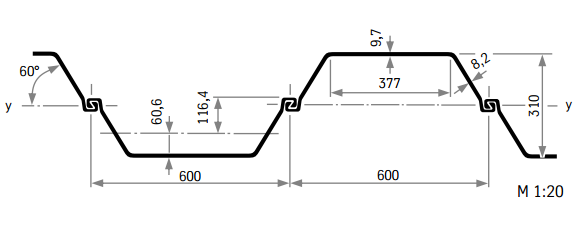
\includegraphics[scale=0.5]{Spundwandschnitt.png}
\caption{Schnitt durch ein Spundwandprofil Larsen 603 \cite[2.1.1 S.10]{spund}}
\end{figure}
\begin{figure}[h!]
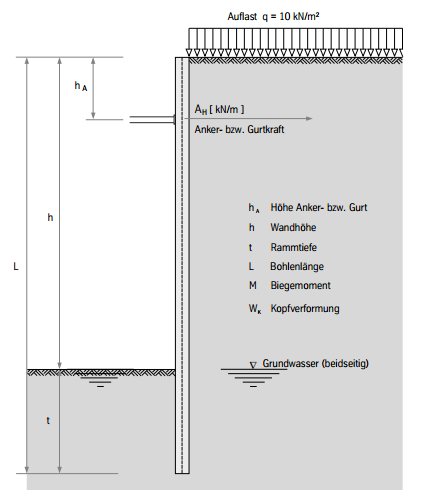
\includegraphics[scale=0.4]{Spundwandlangs.png}
\caption{Längsschnitt durch eine Spundwand \cite[1.6 S.10]{spund}}
\end{figure}
\newpage
\subsubsection*{Variante 2: Gabione}
Gabionen sind mit Steinen gefüllte Drahtkörbe, die zu einer Mauer aufgebaut werden und wie eine Gewichtsmauer wirken. Bei der Füllung ist auf die Auswahl von frost- und Witterungsbeständigem Material zu achten. Die Füllung kann geschüttet werden (wirtschaftlich) oder per Hand gestapelt werden (ästhetisch). Gabionen werden in der Landschaftsarchitektur, im Wasserbau sowie im Straßen- und Wegebau zum Aufbau von Wällen, zur Errichtung von Sicht- oder Lärmschutzanlagen, zur Böschungsbefestigung und als Stützmauer (etwa als Alternative zu konventionellen Trockenmauern in Weinbergen) eingesetzt. \\
Ein Vorteil der Gabionen gegenüber z.B. einer Spundwand ist die gute Anpassungsfähigkeit dem Gelände gegenüber. Außerdem sind sie durch geringen technologischen Aufwand und günstige Baustoffe relativ wirtschaftlich herzustellen. Außerdem sind sie ökologisch nachhaltiger als andere Befestigungen, da sie sich leicht begrünen lassen und so Kleintieren einen Lebensraum bieten können. \\
Früher wurden Gabionen so geplant, dass sie von der Vegetation durchwachsen werden, während gleichzeitig der Draht der Körbe verrostet, sodass wie eine natürliche Befestigung wirkt. Heute werden die Körbe aus verzinktem Stahl gefehrtigt, sodass sie auch mehrere Jahrzente stabil bleiben. Bei grober Fülung der Körbe sind Gabionenwände auch wasserdurchlässig und erhalten so den natürlichen Wasserfluss.\\
Die Herstellung der Gabionenwand ist nicht aufwändig und geht relativ schnell, je nach Qualität des vorhandenen Fundamentes der bisherigen Mauer, sind Betonarbeiten nötig, die den Umfang der Projektes vergrößern.
\begin{figure}[h!]
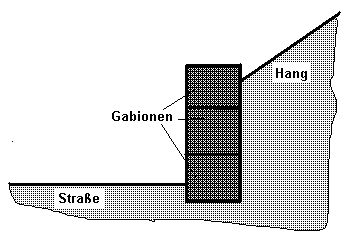
\includegraphics[scale=0.8]{Gabionenwand.png}
\caption{Längsschnitt durch eine Gabionenwand \cite{gabio}}
\end{figure}
\begin{figure}[h!]
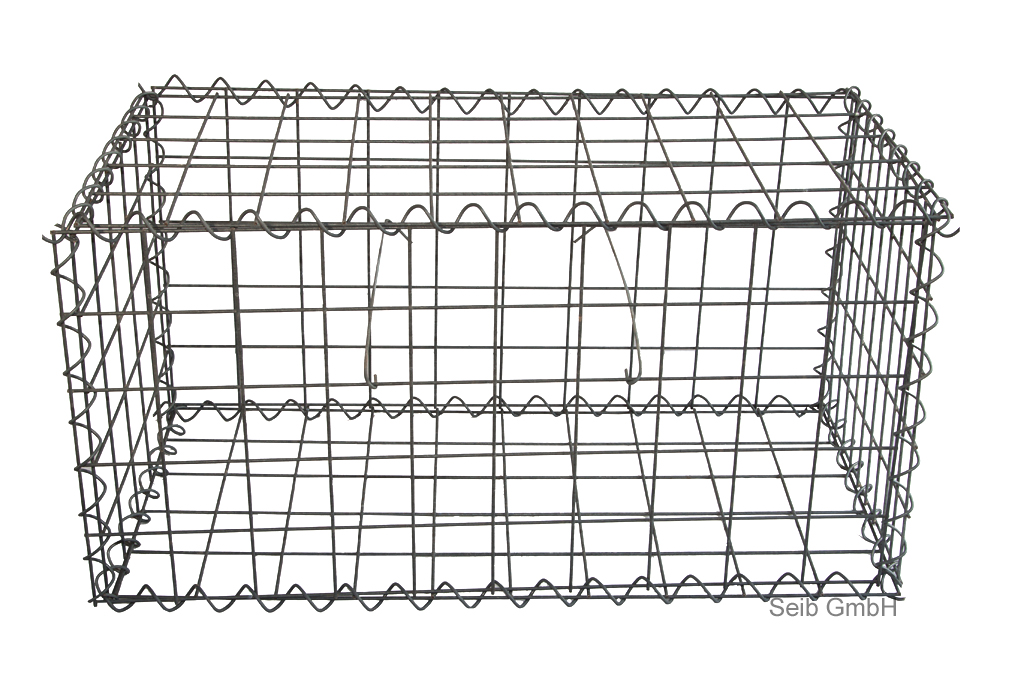
\includegraphics[scale=0.2]{gabione.jpg}
\caption{Ein Gabionenkorb \cite{gabio2}}
\end{figure}
\newpage
\subsubsection*{Variante 3: Gewichtsmauer}
Gewichtsmauern sind massive, meist aus unbewehrtem Beton hergestellte Hangsicherungsbauwerke. Sie gleichen in Bau- und Wirkungsweise den Gewichtsstaumauern aus dem Wasserbau. \\
Gewichtsmauern lassen sich sehr gut an das Gelände anpassen und können auch gut in großen Maßen hergestellt werden. Allerdings brauchen sie relativ viel Material und haben einen relativ langen Herstellungsprozess. Außerdem muss eine Baugrube ausgehoben werden. \\
In der Pflege im Bestand des Bauwerkes sind Betonmauern generell sehr einfach, da Beton ein wetterfestes Material ist.
\begin{figure}[h!]
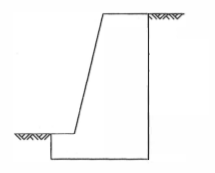
\includegraphics[scale=0.8]{gewichtsmauer.png}
\caption{Längsschnitt durch eine Gewichtsmauer \cite[11.63]{gewichtsmauer}}
\end{figure}
\subsubsection*{Auswahl einer der Varianten}
Jede der drei vorgestellten Varianten hat besondere Vorzüge und ist für bestimmte Szenarien besser geeignet als die anderen. In diesem Fall wähle ich die \textbf{Gabione}. Diese Wahl treffe ich besonders aufgrund des Sickerwassers, das an diesem Hang eintrifft. Bei anderen, wasserundurchlässigen Bauwerken muss sich um die Wasserhaltung gesondert Gedanken gemacht werden und es müssen zusätzliche Entwässerungsanlagen geplant werden. Dies alles ist bei Gabionen nicht der Fall. Weitere Gründe für die Gabione sind eine Tragweise vergleichbar mit der einer Gewichtsmauer, verbunden mit einer Montagegeschwindigkeit, die eher einer Spundwand entspricht. Außerdem kann man dieses Bauwerk sehr gut an die Form des Hanges anpassen. \\
In diesem Fall kommt noch dazu, dass sowohl das Material der vorhandenen Stützmauer als auch der anstehende Boden verwendet werden kann, die Körbe zu befüllen. \\
In meiner Erfahrung sind Gabionen sehr häufig anzutreffende Bauwerke für diesen Zweck. Auch optisch passt eine Gabione besser in die Landschaft einer Wiese, als eine doch sehr massive Stahl- oder Betonkonstruktion.
\subsubsection*{Konstruktiv-technologische Festlegungen}
Aus technologischen Gründen werden Körbe von 1m Höhe, 2m Tiefe und 3m Breite verbaut. Um die nötige Höhe von 3.3m zu überwinden, werden 4 Körbe übereinander gestapelt. Daraus ergibt sich eine Einbindetiefe der Körbe von 70cm. Die Körbe werden wie eine Treppe mit jeweils 30cm Versatz aufeinander gestapelt. Insegesamt ergibt das einen Versatz von 90cm, also einen Wandneigungswinkel von -12.7$^\circ$.\\
Um eine monolithische Wirkung 
Da die Körbe erst vor Ort auf der Baustelle gefüllt werden, wir das vorhandene Material verwendet. Außerdem kann das abgetragene Material der alten Mauer verwendet werden. Allerdings wird die Wichte etwas reduziert angesetzt, da die feinen Anteile aus den Körben heraus rieseln. Ich setze eine Wichte von $16kN/m^3$ an. 
\newpage
\subsubsection*{Bauablauf}
\begin{itemize}
\item Absperrung der Straße
\item Abtragen des Mutterbodens oberhalb
\item Einrammen einer Spundwand als Baugrubensicherung
\item Rückbau der vorhandenen Wand und Abtragen des anstehenden Bodens
\item Ausheben der Baugrube 
\item Aufstellen der Gabionen und lagenweises Hinterfüllen und verdichten des Bodens
\item Nach jeder neuen Lage die Blöcke mit der Lage darunter monolithisch verbinden
\item Bau eines Entwässerungsgrabens entlang der Straße am Fuße der Stützmauer
\item Entfernen der Spundwand und der Absperrung
\item Wiederherstellung der Wiese
\end{itemize}
\subsection{Bemessung}
\subsubsection{Lastannahmen und Lastfälle}
Die einwirkenden Kräfte aus dem Boden ergeben sich aus der Aufgabenstellung. Dazu wird auf der Wiese eine Last von $20kn/m^2$ angesetzt, davon $10kN/m^2$ als ständige Last und $10kN/m^2$ als Verkehrslast.
\subsubsection*{Lastfall aktiver Erddruck und Auflast}
Annahme: $\delta_a = |\alpha| = 12.7^\circ \rightarrow E_{av} = 0 $ \cite[S.149]{wsp}
\begin{equation*}
E_a = E_{ah} =  1/2 \gamma ' h^2 K_{ag} + p h K_{ap} - c h K_{ac}
\end{equation*}
Der Boden hat keine Kohäsion. Deshalb:
\begin{equation*}
E_a = E_{ah} =  1/2 \gamma ' h^2 K_{ag} + p h K_{ap}
\end{equation*}
\begin{equation*}
K_{agh} = \left[\frac{\cos(\varphi - \alpha)}{\cos \alpha \left(1+ \sqrt{\frac{\sin(\varphi + \delta_a)*\sin(\varphi - \beta)}{\cos(\alpha - \beta) * \cos(\alpha + \delta_a)}}\right)}\right]^2
=
\left[\frac{\cos(35^\circ - (-12.7^\circ))}{\cos (-12.7^\circ) \left(1+ \sqrt{\frac{\sin(35^\circ + 12.7^\circ)*\sin(35^\circ - 11^\circ)}{\cos((-12.7^\circ) - 11^\circ) * \cos((-12.7^\circ) + 12.7^\circ)}}\right)}\right]^2 
\end{equation*}
\begin{equation*}
K_{agh} = 0.0.1925
\end{equation*}
\begin{equation*}
K_{aph} = K_{agh}\frac{\cos\alpha \cos\beta}{\cos(\alpha - \beta)} = 0.2013
\end{equation*}
\begin{equation*}
E_a = E_{ah} =  1/2 \gamma ' h^2 K_{ag} + p h K_{ap} = 27.6kN/m
\end{equation*}
\begin{equation*}
y_{E_a} = \frac{2e_{ah1} + e_{ah2}}{e_{ah1} + e_{ah2}} \frac{h}{3} = 1.512m
\end{equation*}
\newpage 
\begin{figure}
\vspace{10cm}
\caption[Erddruckverteilung Aufgabe 1]{Erddruckverteilung \cite{me}}
\end{figure}
\subsubsection{Ermittlung der Einwirkungen}
\begin{equation*}
G_k = Tiefe_{Block} * Höhe_{Block} * Anzahl_{Blöcke} * \gamma_{Block} = 2m * 1m * 4 * 16kN/m^3 = 128kN/m
\end{equation*}
$\hspace{1cm} V_k = 0 $ Aus Annahme für aktiven Erddruck \\
$\hspace{1cm} H_k = 27.6kN/m $ Aktiver Erddruck \\
Schnittgrößen in der Sohlfuge: \\
$\hspace{1cm} N_k = V_k + G_k = 128Kn/m $\\
$\hspace{1cm} T_k = H_k = 27.6kN/m $ \\
$\hspace{1cm} M_k = H_k * y_{E_a} = 27.6kN/m * 1.512m = 41.719kNm/m $ \\
\begin{equation*}
e = \frac{M_k}{N_k} = \frac{41.719kNm/m}{120kN/m} = 0.326m
\end{equation*}
\subsubsection{Nachweis Kippsicherheit GZ EQU}
Berechnungen nach \cite[S.97]{wsp}. Das Verfahren ist anwendbar, da mindestens mitteldicht gelagerter nichtbindiger Boden vorliegt.\\ 
Prüfen, ob die Sohldruckresultierende aus ständigen Belastungen innerhalb der ersten Kernweite liegt: \\
Bedingung: $ e \le b/6 =0.33m$ \\
$ 0.326m \le 0.33m \checkmark$ \\
\newpage
Prüfen, ob die Sohldruckresultierende aus ständigen und veränderlichen Belastungen innerhalb der zweiten Kernweite liegt:\\
Bedingung: $e \le b/3 = 0.66m$\\
Rechnung analog zu nur ständige Einwirkungen.\\
$E_{a,2} = 34.24kN/m$ \\
$M_{k,2} = 44.98kNm/m$ \\
$e_2 = 0.351m \le 0.66m \checkmark$
\subsubsection{Nachweis Grundbruchsicherheit GZ GEO.2}
Berechnung nach \cite[S.99]{wsp}. \\
\textbf{Beanspruchungen:}\\
$V_d = V_G*\gamma_G = 128kN/m * 1.35 = 172.8kN/m$ \\
\\
\textbf{Widerstände}\\
Berechnung der geometrischen Parameter: \\
$ a' = 1m$ Meterstreifen, da Streifenfundament \\
$ b' = b - 2e = 2m - 2*0.326m = 1.348m$ \\
$ \tan\delta = T/N = 0.216 $ \\
$ \delta = 12.55^\circ \rightarrow$ Der Gleitkörper verschiebt sich in Richtung von T. 
\\
Bestimmung des Widerstandes (keine Kohäsion): \\
$R_n = a'b' (\gamma_1 d N_d + \gamma_2 b' N_b)$\\
\\
\begin{tabular}{|l|r|r|}
\hline
 & \multicolumn{1}{l|}{\textbf{Gründungstiefe}} & \multicolumn{1}{l|}{\textbf{Gründungsbreite}} \\ \hline
\textbf{Tragfähigkeit} & 33.296 & 22.614 \\ \hline
\textbf{Form} & 1 & 1 \\ \hline
\textbf{Lastneigung} & 0.615 & 0.483 \\ \hline
\end{tabular}\\
\\
$ N_d = N_{d,0} \upnu_d i_d = 33.296 * 1 * 0.615 = 20.485$ \\
$ N_b = N_{b,0} \upnu_b i_b = 22.614 * 1 * 0.483 = 10.913$ \\
$ R_n = 1 * 1.348 * (20 * 0.7 * 20.485 + 20 * 1.348 * 10.913) = 783.913kN/m$\\
$R_d = R_n/\gamma_{R,v} = 783.913 / 1.4 = 559.938kN/m$ \\
\\
$N_d = 172.8kN/m < R_d = 559.938kN/m$ $\checkmark$ \\
Grundbruchsicherheitsnachweis erfüllt!
\subsection{Konstruktionszeichnungen}
\subsection{Nebenbetrachtungen}

\newpage
\listoffigures
\newpage
\section{Literaturliste}
\begin{thebibliography}{9}
\bibitem[Spundwandhandbuch]{spund} 
http://www.thyssenkrupp-bautechnik.de/fileadmin/Leistungen/01 \_Spundwandprofile/\_media/spundwandhandbuch.pdf
\bibitem[Wikipedia - Gabione]{gabio} http://upload.wikimedia.org/wikipedia/de/3/3b/Gabionenwand.png
\bibitem[Schneider]{gewichtsmauer} Schneider Bautabellen, 20. Auflage
\bibitem[Seib Natursteine GmbH]{gabio2} http://www.seib-natursteine.com/gfx\_content/produktbilder/14030100.jpg
\bibitem[WSP]{wsp} Wissensspeicher Geotechnik - Delef Rütz, Karl Josef Witt - 18.Auflage - Weimar 2011
\bibitem[Paul Debus]{me} Paul Debus - Powered by Faber Castell
\end{thebibliography}

\end{document}
